\section{Methodology}

In the past, software projects followed a strict-plan driven approach, such as the Waterfall method, however more recently, Agile practices have become widely accepted, allowing the developer more freedom. This features an iterative development approach, with short `iterations' or `sprints' defined in which the developer should complete a block of work, typically a `story' or `feature' given the Agile methodology chosen.

The Agile Methodology has a manifesto \cite{Manifesto}, which encompasses all the values it strives to achieve:
\begin{itemize}
  \item \textit{\textbf{Individuals and interactions} over processes and tools}
  \item \textit{\textbf{Working software} over comprehensive documentation}
  \item \textit{\textbf{Customer collaboration} over contract negotiation}
  \item \textit{\textbf{Responding to change} over following a plan}
\end{itemize}

\begin{quotation}
  \textit{That is, while there is value in the items on the right, we value the items on the left more.}
\end{quotation}

Scrum is one of the most popular interpretations of an Agile Methodology, due to its simplicity \cite{scrum}. Scrum is \textit{not} an agile methodology, however it is a framework to which agile practices such as Pair Programming and \acrfull{TDD} can be aligned.

An adapted Scrum methodology has been undertaken for this project. The flexible nature is particularly useful given the research nature of this project, as the requirements were not fully defined at the start of the process, and changed as time went on given the outcome of experimentation with mathematical concepts for image alignment.

Additionally, \acrfull{XP} \cite{xp} dates back to 1996, and is one of the most recognisable Agile Methodologies used in the software industry currently. \acrshort{XP} claims to create successful software projects by following 5 key principles:

\begin{itemize}
  \item \textbf{Communication: } constantly communicate with their customers and fellow programmers
  \item \textbf{Simplicity:} keep the design simple and clean
  \item \textbf{Feedback:} testing the software starting on day one
  \item \textbf{Respect: } every small success deepens their respect for the unique contributions of each and every team member
  \item \textbf{Courage: } deliver the system to the customers as early as possible and implement changes as suggested
\end{itemize}

Given that this project is a single-person project, neither framework/methodology would work well on its own, so for this project it was decided that Scrum would be the main framework, with elements of XP to help strengthen areas such as design and testing.

\subsection{Tools to manage methodology}

This project has been chiefly supported by the application \url{taiga.io} - a beta web app \cite{Taiga.io}, which aims to promote the use of Scrum and Kanban \cite{kanban}.

Having an online application to organise User Stories, Tasks, Issues and to track progress using a Burndown chart was extremely important in this single-person project, where work was carried out across several different devices and platforms. It also ensures a historical record of what was completed, and when, as is evident from Subsubsection \ref{ssec:user-stories}.

\subsection{User stories}
\label{ssec:user-stories}

User Stories are a bid to shift away from talking in technical jargon, and to shift towards talking in plain english about project requirements. When working with a customer, this is obviously useful, as occasionally they are non-technical, so this helps promote an open-dialogue between customer and developer, and a clear understanding of the customer's needs.

User Stories typically follow a template for consistency, usually something similar to:

\begin{quotation}
  \textit{As a $<$type of user$>$, I want $<$some goal$>$ so that $<$some reason$>$.} \cite{user_story}
\end{quotation}

User Stories also have associated Story Points, which is a typically a numbering system leveraged to indicate the effort needed to implement the Story. Due to the uncertain nature of programming, it is not always an accurate reflection of effort, however through the Agile community it is generally accepted that to be consistent in your assignment of points is more useful than being accurate \cite{estimation}. During the early stages of the project estimation can be quite inaccurate, however as the project progresses, and the developer gains a better understanding of the tasks, and how to implement them, then estimation tends to become more accurate.

Table \ref{table:User Stories} outlines the User Stories used during this project, along with when they were worked upon (during which sprint) and how many Story Points were associated with it.

\begin{center}
  \small
  \begin{longtable}{| p{2cm} | p{4cm} | p{2cm}  | p{2cm} | p{3cm} |}
    \hline
      \textbf{Reference} & \textbf{User Story} & \textbf{Milestone} & \textbf{Story Points} & \textbf{Additional Comments} \\ \hline \endhead
      1 & Clinicians can upload a set of images (MATLAB Command Window) so they can control what images are input into the \Gls{Congealing} Algorithm & Sprint 0 & 5 & Initially this was hard-programmed \\ \hline
      2 & Developer will implement membership of a pixel so that Fuzzy Entropy can be calculated & Sprint 1 & 10 & \\ \hline
      3 & Clinicians can align scans using Non-Probabilistic Entropy so it can be used in the \Gls{Congealing} Algorithm & Sprint 2 \& 3 & 20 & Due to complexity of the implementation, this was spread over 2 sprints \\ \hline
      4 & Clinicians can select an alignment metric (MATLAB Command Window) so they can select which to align the images using & Sprint 4 & 5 & \\ \hline
      5 & Developer will make standard GUI with no functionality so that this can be demonstrated as a proof of concept & Sprint 4 & 5 & \\ \hline
      6 & Clinician can choose number of iterations (MATLAB Command Window) so they can run as many as they want to & Sprint 4 & 3 & \\ \hline
      7 & Developer will implement basic mammogram upload so that they can be aligned & Sprint 4 & 8 & \\ \hline
      8 & Clinicians can align scans using Shannon entropy so it can be used in the \Gls{Congealing} Algorithm & Sprint 5 & 8 & \\ \hline
      9 & Clinicians can upload a set of images - GUI & Sprint 5 & 10 & \\ \hline
      10 & Developer will optimise membership function so to improve performance & Sprint 5 & 2 & Promoted from an Issue \\ \hline
      11 & Developer will optimise Non-Probabilistic function so to improve performance & Sprint 5 & 2 & Promoted from an Issue \\ \hline
      12 & Clinicians can clear an input image so that they can reselect an input image - \acrshort{GUI} & Sprint 5 & 3 & \\ \hline
      13 & Clinicians can align scans using Hybrid Entropy so it can be used in the \Gls{Congealing} Algorithm  & Sprint 6 & 20 & \\ \hline
      14 & Clinicians can select an alignment metric from a drop-down menu so it is easy to choose which alignment metric to use - \acrshort{GUI} & Sprint 6 & 5 & \\ \hline
      15 & Clinicians can select the number of iterations to be run using an alignment metric (GUI) so it is easy to select how many iterations to run & Sprint 6 & 5 & \\ \hline
      16 & Clinicians can see metadata about the input image so they can see if the uploaded image is the correct one - \acrshort{GUI} & Sprint 6 & 2 & \\ \hline
      17 & Clinicians can see each iteration mean image so they can compare the improvement over each iteration - \acrshort{GUI} & Sprint 6 & 3 & \\ \hline
      18 & Clinicians can see adjusted input images on final iteration so they can see how the input images have changed by the final iteration - \acrshort{GUI} & Sprint 6 & 3 & \\ \hline
      19 & Developer wants to know why Scans are rotated 90 to left as this is aesthetically displeasing & Sprint 7 & 8 & Promoted from an Issue \\ \hline
      20 & Developer will research and implement removal of Medical Markers as this causes alignment issues & Sprint 7 & 5 & \\ \hline
      21 & Clinicians can discard (clear) an alignment so they can start a new alignment - \acrshort{GUI} & Sprint 8 & 5 & \\ \hline
      22 & Clinicians can click on average image to view it bigger so they can see the detail easier - \acrshort{GUI} & Sprint 8 & 2 & \\ \hline
      23 & Clinicians can save the final mean image with a sensible name so they can easily find it again - \acrshort{GUI} & Sprint 8 & 3 & \\ \hline
      24 & Clinicians can see the iteration details so they can understand more about the improvement - \acrshort{GUI} & Sprint 8 & 8 & \\ \hline
      25 & Clinicians can see \Gls{Congealing} is running so they know it's in progress - \acrshort{GUI} & Sprint 8 & 3 & \\ \hline
  \caption{User stories defined during the project timeline.}
  \label{table:User Stories}
\end{longtable}
\end{center}

\subsection{Burndown chart}

\begin{figure}[H]
  \centering
  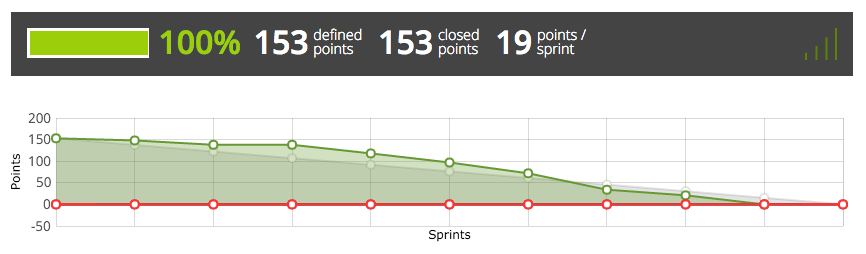
\includegraphics[width=\textwidth]{Chapter2/software-img/burndown.png}
  \caption{Project Burndown chart.}
  \label{fig:burndown}
\end{figure}

Figure \ref{fig:burndown} is a graphical representation of progress per week, as utilised in Scrum, called a Burndown chart. It allows the developer(s) a quick reference as to the progress of the project, and works by subtracting completed Story points as they're completed. Taiga includes the trend line which sets a target for completion per sprint.

In Taiga, it was also possible to have a weekly burndown chart, so as to track progress throughout the week, rather than just the entire project. This ensured a steady rate of development through the week between Supervisor meetings, rather than over-working at the beginning of the week and having nothing left to do at the end, or vice-versa.

\subsection{Sprint review \& retrospective}

Sprint review meetings are held at the end of each sprint, to assess what work was done during the week, and does the end product match the sprint goal set out at the start of the week. In this project, sprint goals, sprint reviews and retrospectives took shape in the form of an informal online blog. sprints were defined as a week long in this project, running between supervisor meetings (Monday - Sunday). Weekly posts would outline what had been completed that week, how things went (good and bad) and what was to be completed during the following week. Whilst less structured than the conventional approach to reviews, it works well within a single-person project, and was a good reflection of what had been accomplished.

In Agile Methodologies, retrospectives are typically at the end of each sprint, so the team can assess:
\begin{itemize}
  \item What works well
  \item What doesn't work well
  \item What should they start doing
\end{itemize}

This ensured good practices were carried forward into the next sprint, whereas unhelpful ideas were left in the previous week.

\subsection{Daily Standup}

Daily standups are a vital part of Scrum`s teamwork ethos. Each morning (or during a set allotted time), the team would meet to discuss what was accomplished the day before, what are the plans for the day ahead, and what road-blocks are in their way. This provides the developer (and furthermore the team) a clear picture of what has yet to be done, and allows fellow team-mates to offer expertise to help overcome obstacles. Whilst this project is not being developed by a team, the benefit of daily standups to productivity, organisation and planning still stands, along with the crowd-sourcing element of expertise.

Throughout the project, stand ups have been held with peers, who are also working on their Major Projects. Whilst not daily, they tended to fall every two days, and it gave the developer a chance to hone skills in explaining the project to people not well-versed in the subject. It was also a good hotbed for new ideas, and an open forum for discussion into the pros and cons of certain approaches.

\newpage
\section{Design}

In traditional plan-driven methodologies, such as the Waterfall method, Design would take shape in the form of a design document where all the requirements would be outlined and written up in detail. As mentioned previously, this would be impractical for such a fluid, experimental project so practices were leveraged from \acrfull{XP} to ensure that the system design was not compromised by the lack of early, solid requirements.

\subsection{CRC Cards}

In \acrshort{XP}, \acrfull{CRC} Cards are useful visual aid so the entire team can easily collaborate on the system design. Whilst there is no team in this project, they still play a vital role in structuring the system, can be iteratively updated and are easily discardable should the need arise.

Typically \acrshort{CRC} cards would represent Objects, with the class written at the top, the responsibilities down the left and the collaborating classes down the right-hand side. However as mentioned in Section \ref{ssec:matlab}, MATLAB is built around a scripting language, and all the `classes' in this project are replaced by functions and scripts. Therefore, each \acrshort{CRC} card represents a function or a script, and its corresponding responsibilities and collaborations as normal - see Figure \ref{fig:crc} for more detail and Appendix \ref{appendix:crc-cards} for the \acrshort{CRC} card iterations throughout the project.

\begin{figure}[H]
  \center
  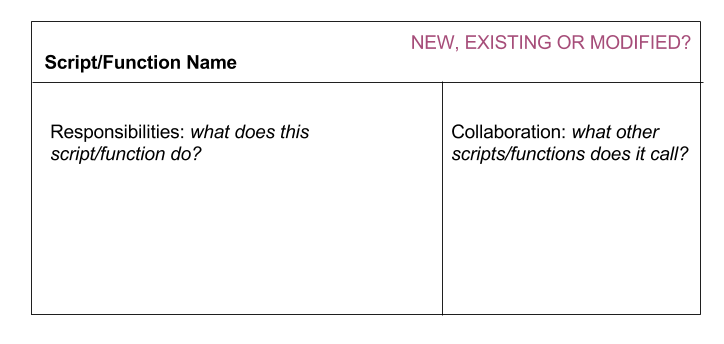
\includegraphics[scale=0.5]{Chapter2/software-img/crc.png}
  \caption{Example CRC Card as used in this project}
  \label{fig:crc}
\end{figure}

\subsection{Graphic User Interface (GUI) Design}
\label{sssec:gui-design}

The name \say{Enantiomorph} was chosen as the application name as a more concise, recognisable alternative to the project title.

\begin{quotation}
  \textit{Enantiomorph: either of a pair of crystals (as of quartz) that are structural mirror images \cite{enantiomorph}}
\end{quotation}

This section will look at the design evolution of the application \acrfull{GUI}.

\begin{figure}[H]
  \center
  \includegraphics[scale=0.5]{Chapter2/software-img/wireframe_1.png}
  \caption{Initial wireframe design for \acrshort{GUI}}
  \label{fig:wireframe1}
\end{figure}

The initial design, as represented in Figure \ref{fig:wireframe1}, was designed to incorporate the first set of project requirements.

\begin{figure}[H]
  \center
  \includegraphics[scale=0.5]{Chapter2/software-img/wireframe_2.png}
  \caption{Second wireframe design for \acrshort{GUI}}
  \label{fig:wireframe2}
\end{figure}

Figure \ref{fig:wireframe2} represents the changes in requirements as the project progressed. It became clear that a load button which allowed the user to \textit{both} generate a large pgm file from a folder of mammograms, or upload a large pgm file that already exists would be difficult to implement. Therefore the button was split into two buttons, with appropriate text above the buttons to help the user decide which to use.

By the second \acrshort{GUI} iteration, it became apparent that implementing a way in which to stop the \Gls{Congealing} algorithm automatically would be too time-consuming for the time left in the project. Therefore the user would have to specify how many iterations they would like to run. This meant a textbox with numerical validation had to be incorporated into the \acrshort{GUI} and the extra iteration information fed into the back-end.

During the second application iteration, the outputs of each iteration mean and the adjusted input images were implemented for the user to see.

\begin{figure}[H]
  \center
  \includegraphics[scale=0.5]{Chapter2/software-img/wireframe_3.png}
  \caption{Third wireframe design for \acrshort{GUI}}
  \label{fig:wireframe3}
\end{figure}
The final wireframe created is outlined in Figure \ref{fig:wireframe3}. Additional information  about the \Gls{Congealing} process can be accessed via the button in the bottom left corner and metadata about the input image displayed in the top section. Users can also clear the entire \acrshort{GUI} to start a new alignment - this could be useful should they wish to compare the outputs from the 3 different entropy alignment techniques.

\noindent \textbf{The final \acrshort{GUI}} can be found in Subsection \ref{ssec:GUI-implement}, Figure \ref{fig:final_gui_pic}.
